\section{Objetivos y preguntas de investigación} \label{sec:research_questions}
En un estudio de carácter exploratorio como el que se propone, definir unos objetivos y preguntas
de investigación se convierte en una tarea fundamental para la correcta orientación del trabajo.
En este sentido, los objetivos nos permiten establecer una serie de metas a alcanzar, mientras
que, las preguntas de investigación nos ayudan a centrar el estudio en aspectos concretos que
queremos responder. Los objetivos de la investigación son los siguientes:

\begin{itemize}
    \item \textbf{OB-1}: implementar un algoritmo de aprendizaje automático que genere un modelo
          predictivo (un \textit{predictor}) basado en un conjunto de características
          \textit{features} extraídas de las \textit{builds}.\\
    \item \textbf{OB-2}: utilizar la \textit{API} de GitHub para obtener datos relevantes sobre
          las \textit{builds}, como su histórico, características asociadas, resultados anteriores
          de la integración continua.\\
    \item \textbf{OB-3}: desarrollar e implementar diferentes algoritmos de predicción con la
          selección de diferentes características con el objetivo de proporcionar múltiples
          opciones a la hora de predecir el resultado de la integración continua.\\
    \item \textbf{OB-4}: implementar una interfaz gráfica que sirva como punto de entrada de
          datos para el algoritmo de predicción y que permita visualizar los resultados
          obtenidos.
\end{itemize}

Antes de introducir las preguntas de investigación, es importante definir el significado de 
algunos términos clave para evaluar el desempeño de los modelos de predicción y la eficacia con
la que cumplen su función. Cuando un algoritmo realiza una predicción, podemos encontrarnos
con cuatro casos:

\begin{itemize}
      \item \textit{True Positive (TP)}: el modelo predice que la \textit{build} fallará y,
            efectivamente, falla.\\
      \item \textit{True Negative (TN)}: el modelo predice que la \textit{build} pasará y,
            efectivamente, pasa.\\
      \item \textit{False Positive (FP)}: el modelo predice que la \textit{build} fallará, pero
            en realidad pasa.\\
      \item \textit{False Negative (FN)}: el modelo predice que la \textit{build} pasará, pero
            en realidad falla.
\end{itemize}


\begin{figure}[H]
      \centering
      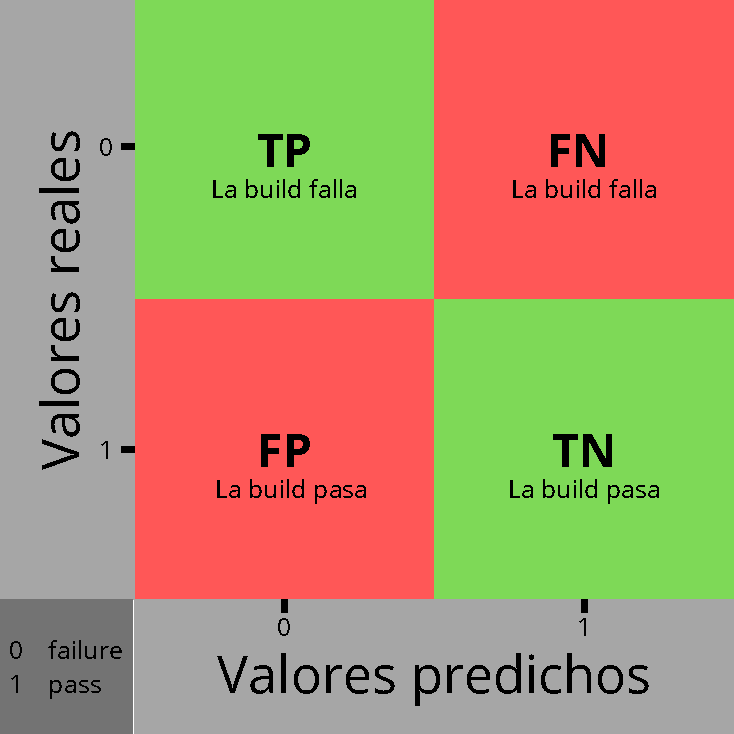
\includegraphics[scale=0.50]{images/Confusion matrix.pdf}
      \caption{Matriz de confusión.}
      \label{fig:confusion_matrix}
  \end{figure}

Con estos conceptos en mente, podemos definir las siguientes métricas de evaluación:

\begin{itemize}
    \item \textit{Accuracy}: mide la proporción de predicciones correctas realizadas por el
          modelo. Se calcula como la suma de los verdaderos positivos y verdaderos negativos
          dividida entre el total de predicciones realizadas.
            \begin{equation}
                  ACC = \frac{TP + TN}{TP + TN + FP + FN}
            \end{equation}
    \item \textit{Precision}: mide la proporción de predicciones positivas correctas realizadas
          por el modelo. Se calcula como la suma de los verdaderos positivos dividida entre la
          suma de los verdaderos positivos y falsos positivos.
            \begin{equation}
                  P = \frac{TP}{TP + FP}
            \end{equation}
    \item \textit{Recall}: mide la proporción de instancias positivas que el modelo predice
          correctamente. Se calcula como la suma de los verdaderos positivos dividida entre la
          suma de los verdaderos positivos y falsos negativos.
            \begin{equation}
                  R = \frac{TP}{TP + FN}
            \end{equation}
    \item \textit{F1-score}: es la media armónica de \textit{precision} y \textit{recall}.
            \begin{equation}
                  F1 = 2 \times \frac{P \times R}{P + R}
            \end{equation}
\end{itemize}

Las preguntas de investigación delimitan el alcance del estudio y ayudan a enfocar el trabajo en
aspectos específicos del tema a investigar, evitando que nos desviemos hacia otras áreas no
relevantes. Ayudan a clarificar qué se quiere lograr con la investigación y guían en el proceso
metodológico, es decir, dependiendo de las preguntas de investigación, podremos determinar
si necesitamos una metodología cuantitativa, cualitativa o mixta. Además, estas tienen una
función estructutural, ya que las secciones y capítulos siempre irán orientados a responder
estas preguntas. A continuación se detallan las preguntas de investigación junto a las
métricas usadas para su evaluación:


\begin{itemize}
    \item \textbf{PI-1}: ¿Qué algoritmo de predicción produce los mejores resultados en la
          predicción automática del resultado de la integración continua?\\
          \begin{itemize}
            \item \textbf{Métrica}: \textit{accuracy}, \textit{precision}, \textit{recall} y
                  \textit{F1-score} del modelo.\\
          \end{itemize}

    \item \textbf{PI-2}: ¿Qué características de las \textit{builds} son más significativas en
          la predicción?\\

          \begin{itemize}
            \item \textbf{Métrica}: importancia de cada \textit{feature} a través de la
            interpretación de los coeficientes del modelo.
          \end{itemize}
\end{itemize}

Finalmente, queda mencionar que en un modelo entrenado con una serie de \textit{features}, los
coeficientes del modelo representan la relación cuantitativa entre cada \textit{feature} y la
variable objetivo, en este caso, la predicción del resultado de la \textit{build}. Por tanto, los
coeficientes indican cómo se espera que cambie el valor de la predicción cuando la correspondiente
\textit{feature} cambia, manteniendo constante el resto de características.